\documentclass[11pt,a4paper,twoside,openany]{book}
\usepackage[nologo]{thesds}
% \usepackage[nologo]{thesds} % ロゴを非表示
% \usepackage[english]{thesds} % for English

% 図が多くビルドに時間がかかるときは
% \documentclass[12pt,a4paper,twoside,openany,draft]{book}
% のように\documentarticleのオプションに「draft」を追加する

% ***** フォントについて *****
% フォントに関しては原ノ味フォント, Roboto, STIX Twoを使用しています。
% もしフォントがないという警告が出る場合には事前に各自の環境にインストールしてください。
% なお、日本語の部分には斜体は使えないので注意してください。
% 原ノ味フォント: https://github.com/trueroad/HaranoAjiFonts
% Roboto: https://fonts.google.com/specimen/Roboto
% STIX Two Text: https://fonts.google.com/specimen/STIX+Two+Text

% ***** 追加のパッケージ *****
% !注意!
% グラフィクス用のpackageは既にusepackageしているので、
% \usepackage[dvips]{graphics}などと書くとエラーになる
\usepackage{amsmath}
\usepackage{amssymb}
\usepackage{amsthm}
\usepackage{mathtools}
\usepackage{url}
\usepackage{array}
\usepackage{siunitx}

% ***** テーブル用のパッケージ *****
\usepackage{tabularray}
\UseTblrLibrary{booktabs,siunitx}

% ***** 数式をキレイにするパッケージ *****
\usepackage{physics2}
\usephysicsmodule{ab}

% ***** argmin, argmax *****
\DeclareMathOperator*{\argmax}{argmax}
\DeclareMathOperator*{\argmin}{argmin}


% ***** BibTeXの設定 *****
\usepackage[
  backend=biber,
  backref=true,
  sortcites=true,
  style=ieee,
  citestyle=numeric,
  maxbibnames=999,
  mincitenames=999,
  maxcitenames=999,
  sorting=none,
  url=false,
  doi=true,
  isbn=true
]{biblatex}

% backrefの表記を編集
\DefineBibliographyStrings{english}{%
  backrefpage = {cited on page},    % originally "cited on page"
  backrefpages = {cited on pages},  % originally "cited on pages"
}

% 余計な項目を非表示にしておく (必要な場合はコメントアウトする)
\AtEveryBibitem{
  \clearfield{eprint}%
  \clearfield{date}%
  \clearfield{month}%
  \clearfield{issn}%
  \clearfield{series}%
  \clearlist{address}%

  % "book"以外から削除する項目
  \ifentrytype{book}{}{
    \clearfield{isbn}%
    \clearname{editor}%
    \clearlist{publisher}%
  }
}

% BibTeXのソースを指定
\addbibresource{references.bib}

% ***** 画像を入れるフォルダの設定 *****
\graphicspath{{figs}}

% ***** タイトルページ *****
\thesistype{令和6年度~修士論文}
\title{卒業・修了論文の書き方}
\author{山田 太郎}  % 自分の名前
\affiliation{一橋大学大学院 ソーシャル・データサイエンス研究科 修士課程}
\date{2025年3月 提出}
% 英語の情報 (日本語の場合には不要)
\etitle{How to Write a Graduation Thesis}
\eauthor{Taro Yamada}  % 自分の名前 (英語)
\eaffiliation{Graduate of Social Data Science\\Hitotsubashi University}
\edate{March, 2025}
% 日本語タイトルと英語タイトルの間のスペース
\adjustspace{100truept}

% ------------------------------------------------------------------------------
% 実際の文章の開始
% ------------------------------------------------------------------------------
\begin{document}

% ***** 表紙を出力 *****
\frontmatter
\maketitle

% ***** 論文全体の概要 *****
\begin{abstract}
  論文全体の概要を書く。概要は、論文全体の内容がイメージできるものである必要があるので、提案法についてだけでなく、研究背景や、提案法に至る着想、提案法の中身、実験結果、展望も含め全体について簡潔に書くことを心がける。その際、多くのことを主張することは避けて、論文の最も重要な部分、例えば、研究上の新規性であったり、提案法により得られた有効な結果について重点的に述べる。時折、やたら研究背景が長く書いてある概要を見かけるが、最低でも自分が研究したことが半分以上は概要に入るようにする。 \\
  
  Write the abstract here. As the abstract should provide an overview of the whole thesis, you should include brief descriptions of the entire contents, i.e., background, inspiration, proposed method, experimental results, and future spectacular. Then, you should avoid claiming too many things. You should focus on important perspectives of the thesis, for instance, the research novelty and main findings offered by the proposed method. Some students write too much research background in the abstract, but it is not preferable. You should write what you did in at least one-half of the abstract.
\end{abstract}

% ***** 目次たち *****
\tableofcontents  % 目次
\clearpage

\listoffigures    % 図目次
\clearpage

\listoftables     % 表目次
\clearpage

% ------------------------------------------------------------------------------
% 本文の開始
% ------------------------------------------------------------------------------
\mainmatter

% 章ごとにファイルを分割すると良い
% ルートのディレクトリが散らからないようにサブフォルダに入れる
% 全体をコンパイルするには時間がかかるので執筆時は適宜、以下をコメントアウトする
\chapter{\latex の基本}
\label{chap:latex-basic}

\begin{chapabst}
  章の概要を別にして書きたい場合には「\texttt{chapabst}」コマンド (pethesis.styで定義) を使う。\texttt{chapabst}コマンドを使わない場合、章の概要は表示されない。
\end{chapabst}

\latex を解説している文章は世の中にたくさんあると思われるが、比較的まとまっているのは「Wikibook」にある「LaTeX」の項目だろう。英語だが、平易に書かれており、\latex のソースコードも多く示されているので、読むのに苦労することは少ないと思われる (一応、日本語版もあるが、やや量が少ない)。\latex の基本的な書き方で分からないことがあれば、まずはここを参照すること。
\begin{itemize}
  \item \textsf{Wikibook: LaTeX}~~(\url{https://en.wikibooks.org/wiki/LaTeX})
\end{itemize}

この章では、\cref{sec:write-equation}で式の書き方を、\cref{sec:insert-figure}では図の入れ方を、\cref{sec:insert-table}では表の入れ方を、\cref{sec:write-algorithm}ではアルゴリズムの書き方を、最後の\cref{sec:cite-articles}では文献引用の方法について述べる。

% ------------------------------------------------------------------------------
\section{式の書き方}
\label{sec:write-equation}
% ------------------------------------------------------------------------------

式には主に文中に式を代入するやり方と、横いっぱいの領域に式を入れる方法の二つがあり、前者の方法を特にインラインと呼ぶこともある。例えば、二次方程式を解く場合、多項式の係数を$a, b, c$とすると、一般的な二次方程式は以下のように書ける。
%
\begin{equation}
  a x^2 + b x^2 + c = 0.
  \label{eq:quadratic-equation}
\end{equation}
%
式を書いた後に空白行をいれると、段落が変わったものと見なされてしまうので、通常はこのように\texttt{\textbackslash end\{equation\}}の後に続けて文章を書くか、「\%」を間の空行に入れることで改段落を防げる。また、論文において、式は文章の一部とみなされるため、一般的には、式の最後にピリオドあるいはコンマをつける。

式を引用する際は\texttt{cleveref}の機能を使って\texttt{\textbackslash cref\{eq:quadratic-equation\}}のように書く。出力は\cref{eq:quadratic-equation}のようになる。\texttt{\textbackslash cref}は式だけでなく図や表にも同じように使えて、自動的に図、表と言ったラベルが切り替わる。また、複数の式を一度に引用する場合には\texttt{\textbackslash cref\{eq:quadratic-equation,eq:with-align\}}のようにコンマで区切ると、「\cref{eq:quadratic-equation,eq:with-align,eq:with-gather}」のように、自動的にそれらしい表記に変換してくれる (コンマとラベルの間にスペースは入れられない)。また連続した番号を物色を引用すると、「\cref{eq:example-line-1,eq:example-line-2,eq:with-align,eq:with-gather}」のように表記される。

数式を複数行で表示する時、かつては\texttt{eqnarray}を使うことが多かったが、最近は\texttt{align}あるいは\texttt{gather}を使うのが一般的。\texttt{align}の場合、\texttt{eqnarray}と同様、式を揃える時には\&を使う。
%
\begin{align}
  a &= a', & b &= b', & c &= c', \label{eq:example-line-1} \\
  a &= a', & b &= b', & c &= c'. \label{eq:example-line-2}
\end{align}
%
一方で\texttt{gather}は式を\&の位置で揃えるのではなく、各行を中央ぞろえにする。
%
\begin{titlebox}{\texttt{align}を使った場合}
  \adjustdisplayskips{1mm}
  \begin{align}
    \mathbf{x} = \argmin_{\mathbf{x}} \| \mathbf{Ax} - \mathbf{b} \|^2 \nonumber \\
    \mbox{where} \quad \mathbf{A} \in \mathbb{R}^{n \times m}, \quad \mathbf{b} \in \mathbb{R}^n \label{eq:with-align}
  \end{align}
\end{titlebox}
%
\begin{titlebox}{\texttt{gather}を使った場合}
  \adjustdisplayskips{1mm}
  \begin{gather}
    \mathbf{x} = \argmin_{\mathbf{x}} \| \mathbf{Ax} - \mathbf{b} \|^2 \nonumber \\
    \mbox{where} \quad \mathbf{A} \in \mathbb{R}^{n \times m}, \quad \mathbf{b} \in \mathbb{R}^n \label{eq:with-gather}
  \end{gather}
\end{titlebox}
%
上記の二つの式で\cref{eq:with-align}が\texttt{align}を使ったもの、\cref{eq:with-gather}が\texttt{gather}を使ったものである。

なお、ベクトルや行列の表記についてだが、計算機科学の分野では「Numerical Recipes in C」~\cite{numrecipes}という本の書き方に倣い、ベクトルを$\mathbf{x}$のようなアルファベット小文字のボールド体、行列を$\mathbf{A}$のようなアルファベット大文字のボールド体で書く。応用数学の分野などでは斜体かつボールドでない文字を使う文化もあるが、$\bm{x}$のようなイタリック・ボールド体はあまり使わないので注意。

\subsection{数式の例いろいろ}

\begin{titlebox}{積分}
  \adjustdisplayskips{1mm}
  \begin{equation}
    I = \int_0^{\infty} x^2 \mathrm{d}x
  \end{equation}
  \begin{center}
    ※ $dx$は正式には$\mathrm{d}x$のように$d$を斜体にせずに書く
  \end{center}
\end{titlebox}

\begin{titlebox}{和の計算}
  \adjustdisplayskips{1mm}
  \begin{equation}
    S = \sum_{i=0}^N x^2
  \end{equation}
\end{titlebox}

\begin{titlebox}{行列}
  \adjustdisplayskips{1mm}
  \begin{equation}
    \mathbf{A} = \begin{bmatrix}
      a_{0,0} & a_{0,1} & \cdots & a_{0,n-1} \\
      a_{1,0} & a_{1,1} & \cdots & a_{1,n-1} \\
      \vdots & \vdots & \ddots & \vdots \\
      a_{n-1,0} & a_{n-1,1} & \cdots & a_{n-1,n-1}
    \end{bmatrix}
  \end{equation}
\end{titlebox}

% ------------------------------------------------------------------------------
\section{数値や単位の書き方}
\label{sec:numbers-and-units}
% ------------------------------------------------------------------------------

数値や単位を書く場合は、通常通り数字を書けば問題ないが、\texttt{siunitx}パッケージを使うと便利な場合がある。例えば、有効数字を明らかにして$1.0 \times 10^3$のように書く場合、数式モードで書き下しても良いが、\texttt{siunitx}を用いると\texttt{\textbackslash num\{1.0e3\}}のように書くだけで「\num{1.0e3}」と出力される。またコンマで3桁ごとに区切られた数字も\texttt{siunitx}を用いることで\num{1000000} (\textbackslash num\{1000000\})のように書くことができる (\texttt{pethesis.sty}ファイルにて\texttt{\textbackslash sisetup\{group-separator=\{,\}\}}を指定している)。

単位を付ける場合には、チルダ記号「$\sim$」を使って数字と単位の間に半角スペースを入れ、10~kVのように書く。このような単位付きの表記の場合も、同様に\texttt{siunitx}パッケージを使うと便利な場合がある。同じ出力は\texttt{\textbackslash qty\{10\}\{\textbackslash kV\}}のように書くと得られ、出力は「\qty{10}{\kV}」のようになる。特に$\mathrm{\mu m}$のようにギリシャ文字が含まれるような単位は\texttt{\textbackslash qty\{10\}\{\textbackslash um\}} (出力: \qty{10}{\um})のように書く方がフォントを揃えるのが容易である。この他にも様々な単位が事前定義されているので、詳しくはドキュメントを確認すると良い。なお、角度の記号などはスペースを入れずに書くのが通例で、\texttt{siunitx}では\texttt{\textbackslash ang\{90.0\}}のように書くことで、「\ang{90.0}」という出力が得られる。

% ------------------------------------------------------------------------------
\section{図の入れ方}
\label{sec:insert-figure}
% ------------------------------------------------------------------------------

一昔前は日本語を\latex で使うために「pLaTeX」+「dvipdfmx」を使う必要があり、一度中間のDVIファイルを作る都合から画像ファイルをEPS形式で要する必要があった。 一方、現在は\pdflatex のほか\lualatex や\xelatex など、DVIを介せずに直接PDFを出力できる\tex を使用するため、画像はPDFファイルとして用意するのが一般的である。JPEGファイルを直接取り込むことも可能であるが、できる限りPDFで用意することを推奨する。

画像の取り込みには\texttt{figure}環境と\texttt{includegraphics}命令を以下のように組み合わせる。結果は\cref{fig:remeshing}のようになる。なお、本テンプレートは画像のPDFファイルを\texttt{figs}フォルダに配置しているが\texttt{pethesis.tex}のプリアンブルに\texttt{graphicspath}を指定しているため、このフォルダの中に画像ファイルが入っている場合には、フォルダを別段指定する必要はない。

\begin{lstlisting}[language=tex,caption={図の貼り方}]
  \begin{figure}[tb]
    \centering
    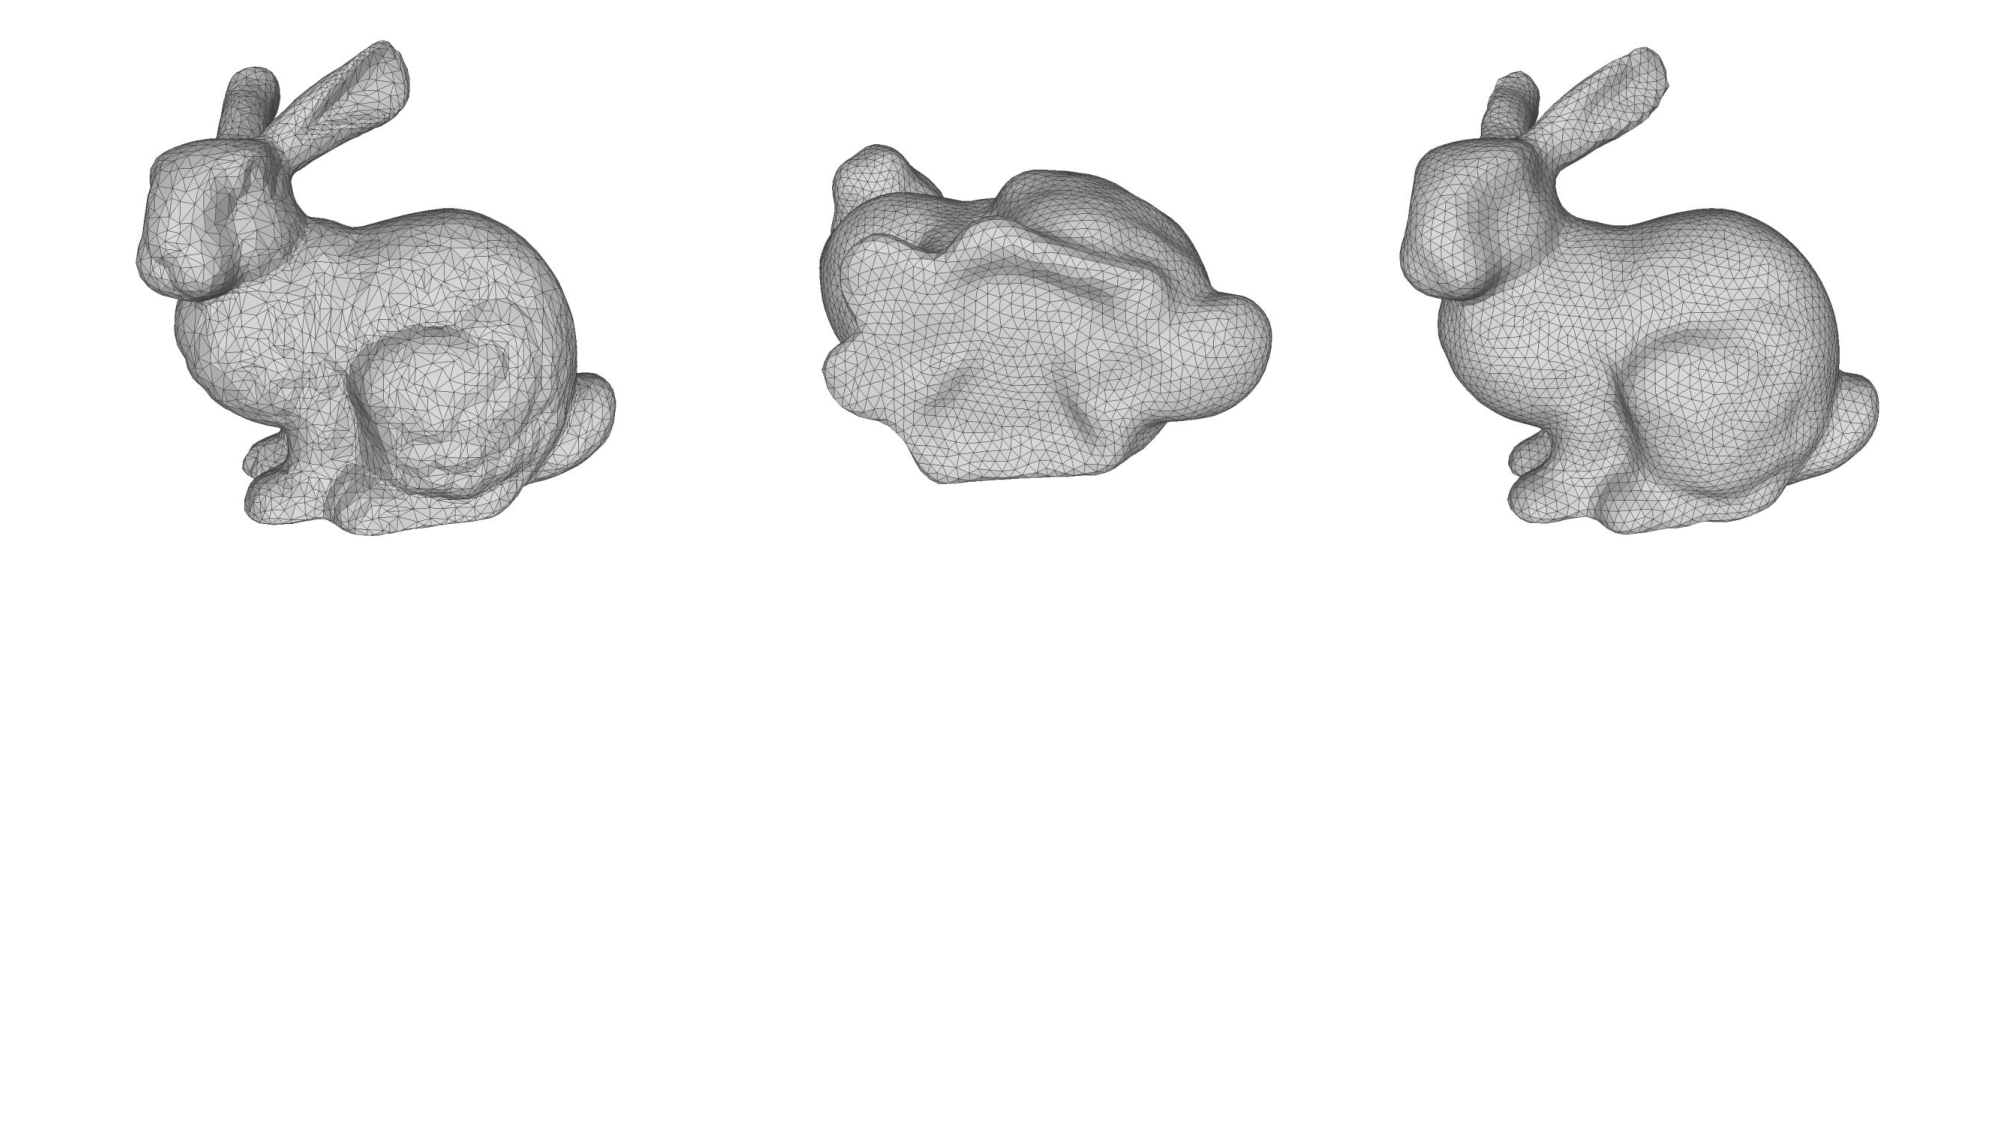
\includegraphics[width=\linewidth]{triangulation}
    \caption{Stanford bunnyモデルのリメッシュ結果}
    \label{fig:remeshing}
  \end{figure}  
\end{lstlisting}

\begin{figure}[!h]
  \centering
  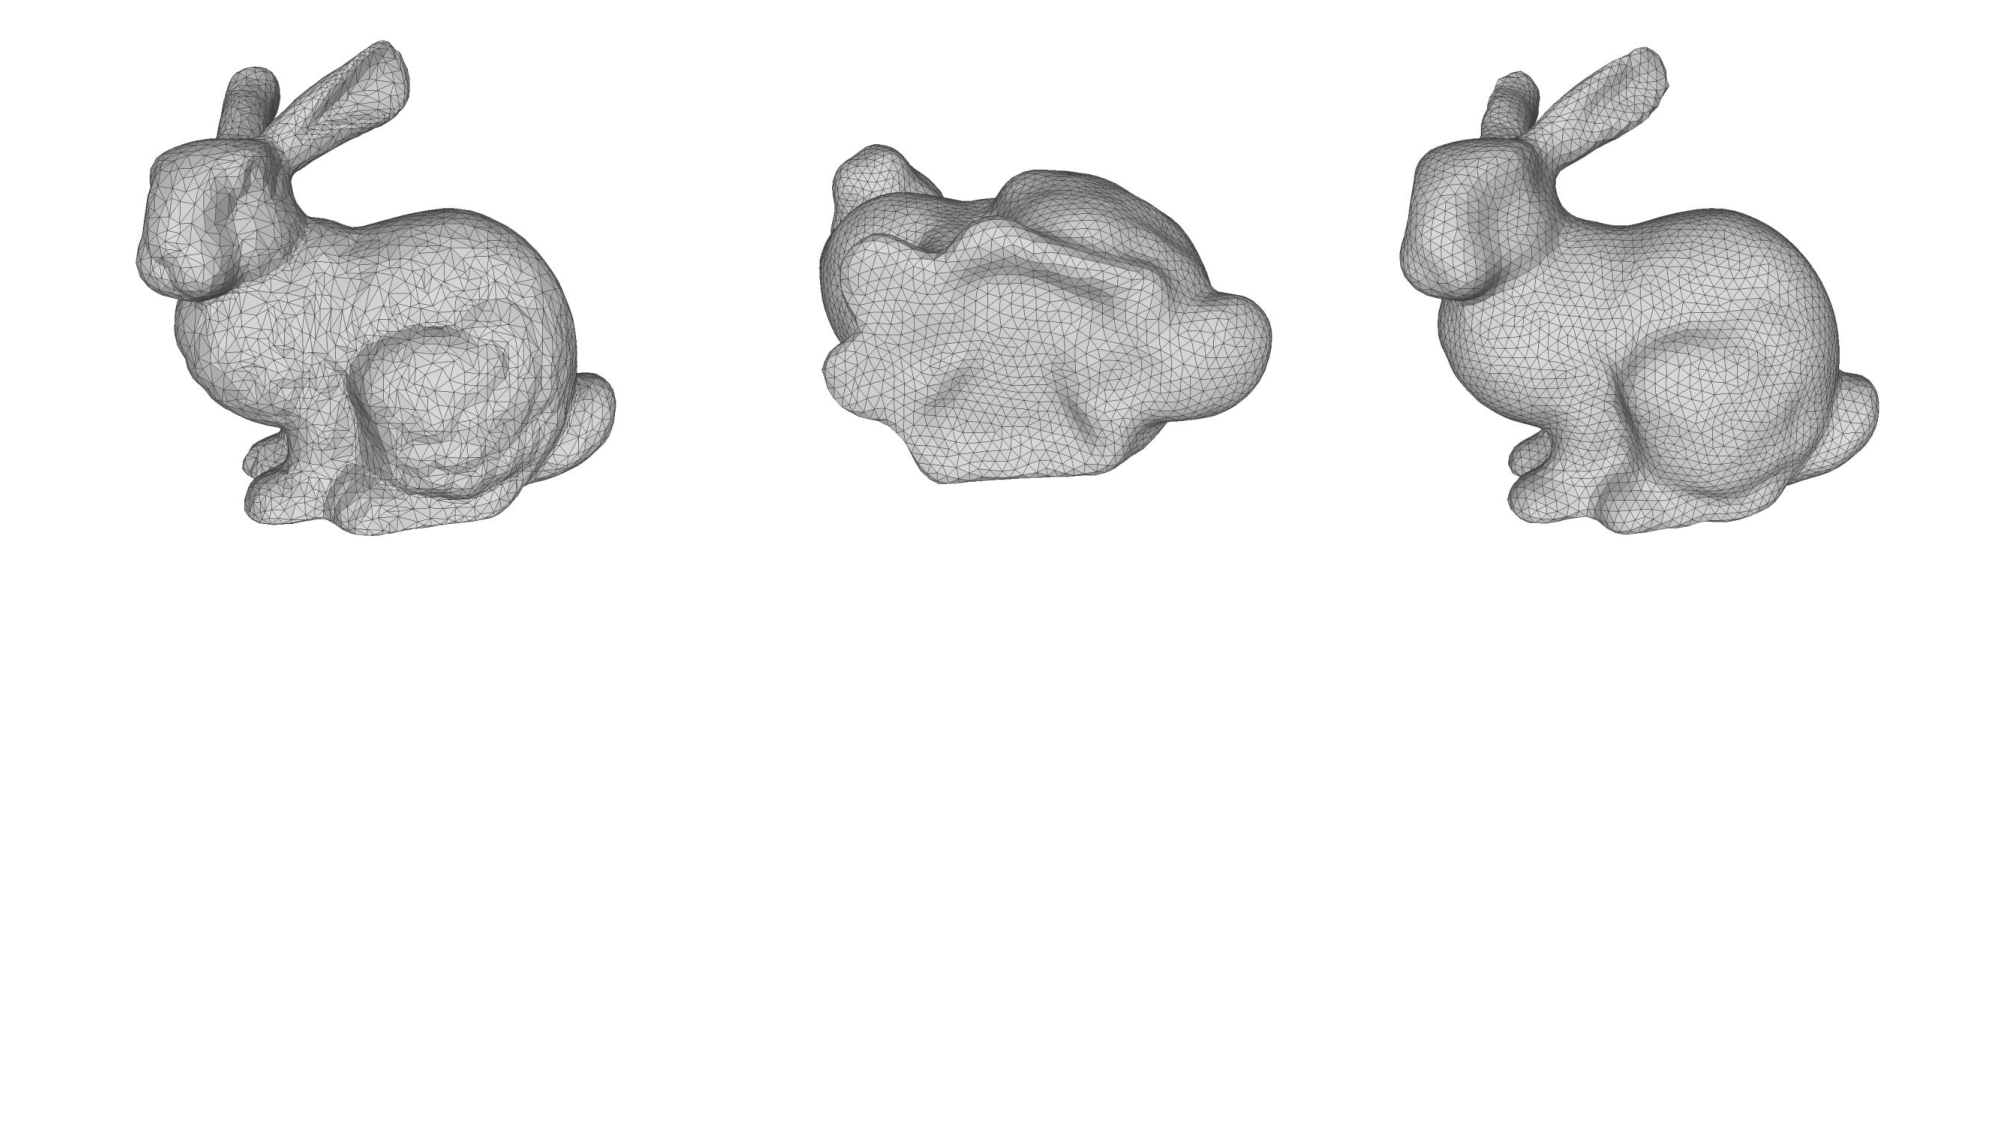
\includegraphics[width=\linewidth]{triangulation}
  \caption{Stanford bunnyモデルのリメッシュ結果}
  \label{fig:remeshing}
\end{figure}

\begin{figure}[tbp]
	\centering
	\begin{tabular}{ccc}
    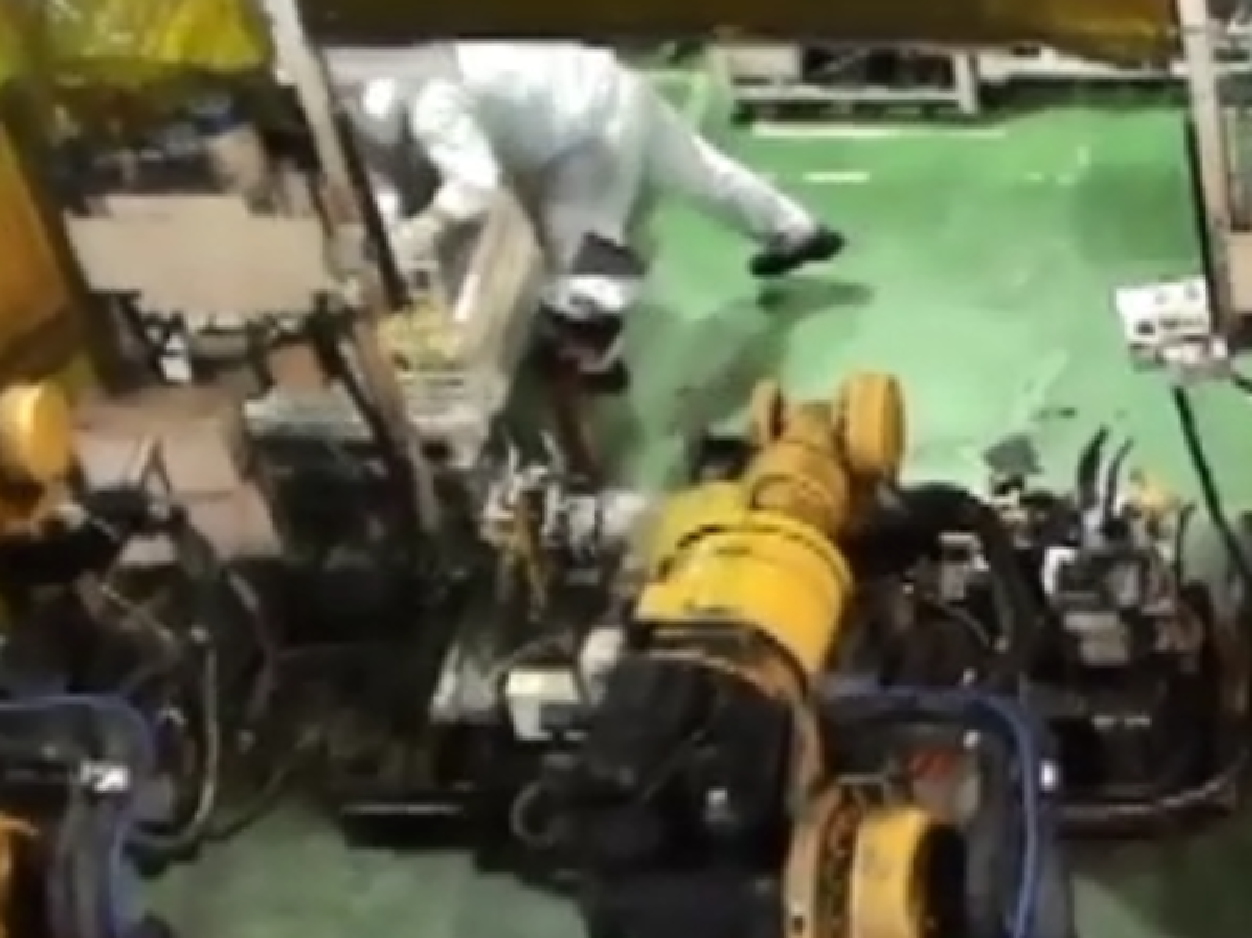
\includegraphics[width=.3\linewidth]{gtekt1} &
    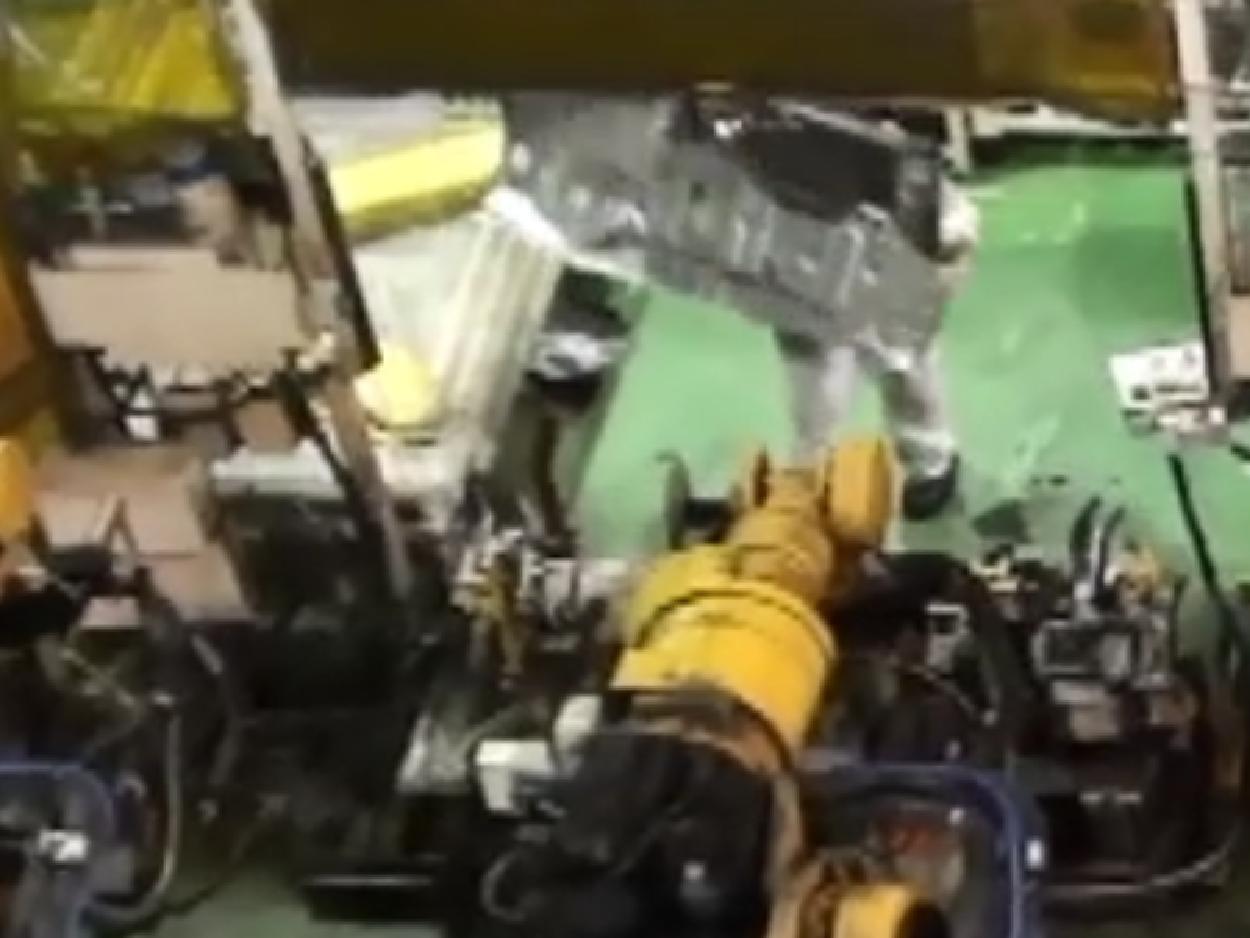
\includegraphics[width=.3\linewidth]{gtekt2} &
    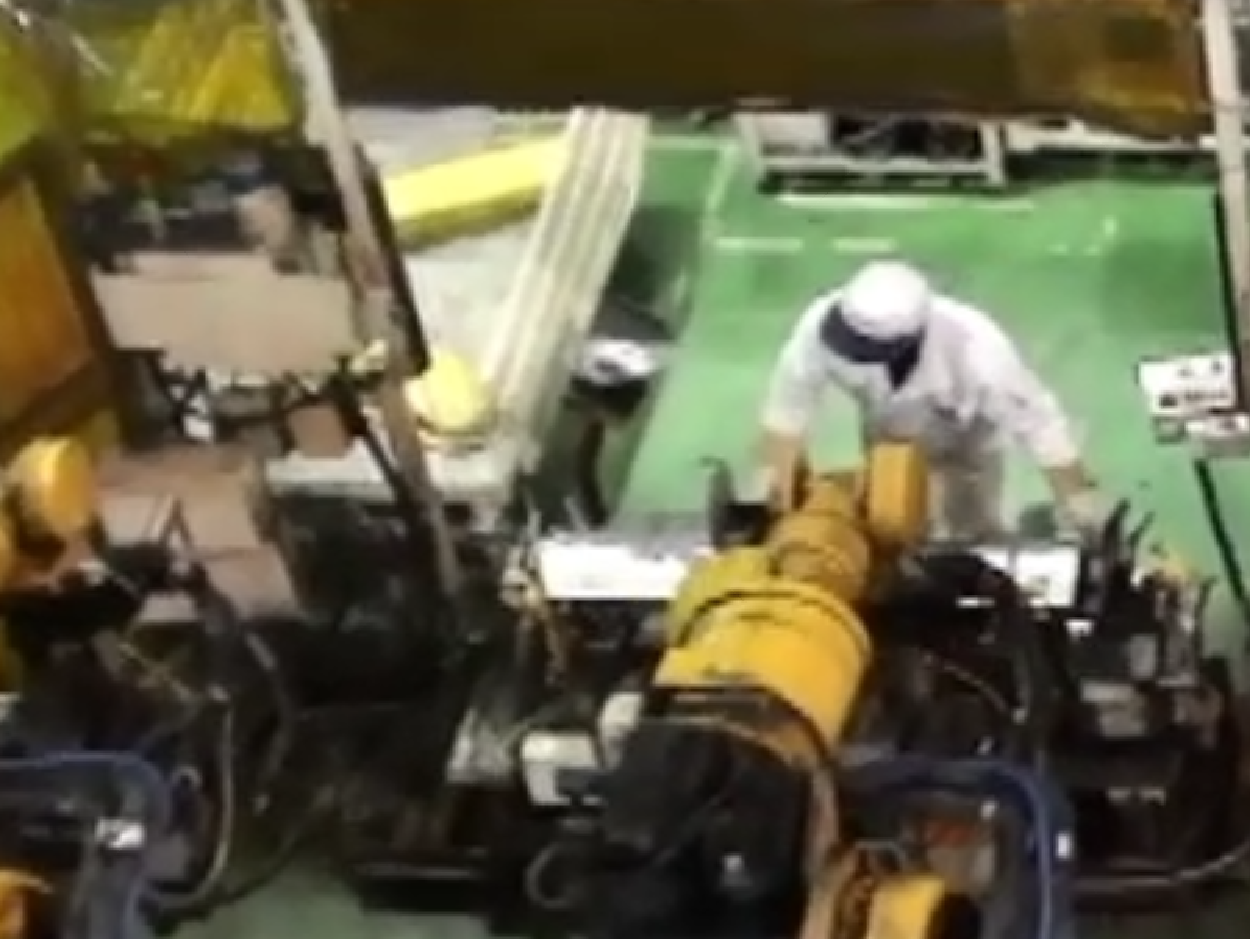
\includegraphics[width=.3\linewidth]{gtekt3}
  \end{tabular}
	\caption[溶接工程における大型部品運搬の様子]{溶接工程における大型部品運搬の様子 (図は株式会社ジーテクトのウェブページ~\cite{GTekt}より引用)}
	\label{fig:welding}
\end{figure}

また、複数の図を\cref{fig:welding}のような形で、\texttt{figure}と\texttt{tabular}を使ってレイアウトすることもできるが、図のレイアウトの自由度が低く、図の間のスペースが広くなる傾向にあるので、個人的にはおすすめはしない。なるべく、一枚の図を作って取り込む方が見た目はきれいになる。

図の配置については、通常、図はページの上に揃えて配置することが一般的であるので\texttt{\textbackslash \{figure\}[t]}のような形でtopに揃えることを意味するtを添えることが多い。この他、図が下に揃ってもいい場合には「b」、図を1ページを丸々使って表示したい場合には「p」を指定する。その場に表示したい場合には「h」あるいは「!h」を指定すればよいが、通常あまり好ましくないとされている。

キャプションを書く際、特に図目次がある学位論文においては、キャプションが長いせいで図目次が見づらくなることがある。この場合は、\texttt{\textbackslash caption[図目次用のキャプション]\{図の下に出るキャプション\}}のように書くことで、図目次専用のキャプションを指定できる。

% -----------------------------------------------
\subsection{図を入れる際の注意事項}

\begin{figure}[tbp]
  \centering
  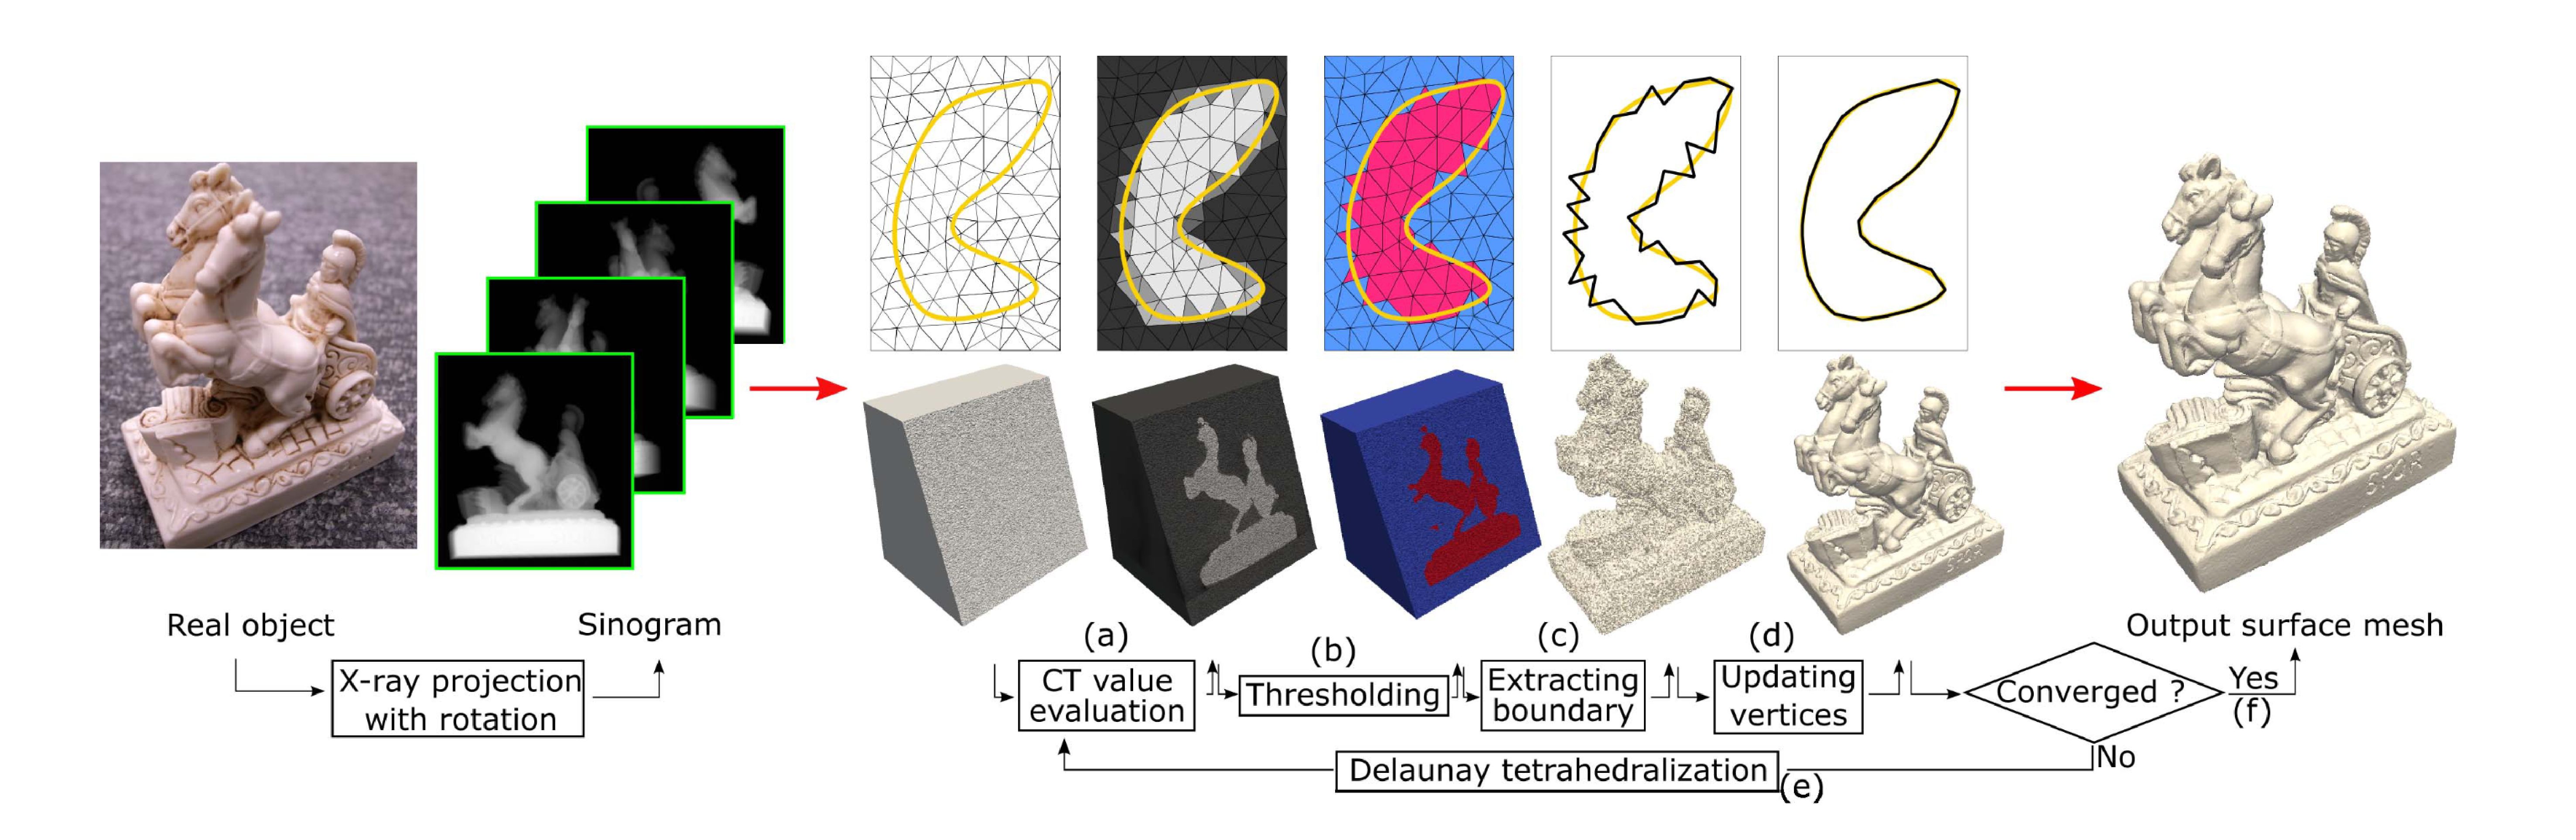
\includegraphics[width=\linewidth]{sinogram_polygonizer}
  \caption[Sinogram Polygonizer法の概念図]{Sinogram Polygonizer法の概念図 (Yamanaka et al.~\cite{yamanaka2013sinogram}, \copyright 2013 IEEE)。}
  \label{fig:sinogram-polygonizer}
\end{figure}

図を別の論文から直接貼り付けることは一般的には好ましくなく、学会や論文誌に投稿する論文においては、ほとんどなされることはない。ただし、書籍や学位論文においては、一定のルールの元で引用することは可能と考えられている。厳密には、画像の著作権を有する学会や個人に許可をとった上で、掲載料を払って掲載する。主要な学会ではIEEEなどは学位論文に関しては掲載料が無料だが、ACMはかなり高額な掲載料がかかるので、特に一般に閲覧可能となる博士論文などは正規の手続きが求められる。引用に際しては\cref{fig:sinogram-polygonizer}のように、図のキャプションに論文のコピーライトを掲載する。


% ------------------------------------------------------------------------------
\section{表の書き方}
\label{sec:insert-table}
% ------------------------------------------------------------------------------

表の書き方については詳しく触れないが、テーブルの間の罫線については\texttt{\textbackslash hline}ではなく、\texttt{booktabs}パッケージの\texttt{\textbackslash toprule} (テーブルの上端の線)、\texttt{\textbackslash midrule} (テーブルの中間に使う線)、\texttt{\textbackslash bottomrule}のように太さが異なる線を使う方が見やすい。特に近年のCG分野の研究では、縦線を使うことはほとんどなく、\texttt{\textbackslash cmidrule} を使ってテーブルの横線に切れ目を入れることで区別をする場合が多いように感じる。

加えてテーブルの横幅だが、最近は\cref{tab:num-fruits-tblr}のようにページの幅いっぱいにテーブルを広げているものを多く見る。テーブルを横方向一杯に広げる方法はいくつかあるが、最も簡単なのは\texttt{tabularray}パッケージを使う方法である。\texttt{tabularray}パッケージでは、「\texttt{\textbackslash begin\{tblr\}\{colspec=\{列フォーマット指定\}, width=\textbackslash linewidth\}}」のように書くことでテーブルの幅を指定できる他、列のフォーマット指定時に「\texttt{lcr}」などの代わりに\texttt{X[l]}, \texttt{X[c]}, \texttt{X[r]}のように書くことで、テーブルの幅を保ったまま、各列の文字揃えを指定できる。これ以外にも、\texttt{{X[2,l]X[1,c]X[1,c]}}のように指定することで、各列の幅の比 (この例では2:1:1)などを指定することもできる。ただし、\texttt{tabularray}パッケージは\latex 3でないと使えないので注意。

\begin{itemize}
  \item \textsf{Package tabularray --- CTAN} \\(\url{https://www.ctan.org/pkg/tabularray})
\end{itemize}


\begin{table}[tb]
  \centering
  \caption{\texttt{tblr}環境を使った場合。}
  \label{tab:num-fruits-tblr}
  \begin{tblr}{colspec={X[2,r]X[3,c]X[3,c]X[3,c]}, width=\linewidth}
    \toprule
    名前 & りんご & みかん & バナナ \\
    \cmidrule{1-1} \cmidrule[l]{2-4}  % tabularrayの場合は()が[]に変わるので注意
    個数 & 1個 & 2個 & 3個 \\
    \bottomrule
  \end{tblr}
\end{table}

\begin{table}[tb]
  \centering
  \caption{列の幅を個別に指定した場合。}
  \label{tab:num-fruits-tabular}
  \begin{tblr}{
    column{1}={0.15\linewidth,r},
    column{2,3,4}={0.22\linewidth,c}
  }
    \toprule
    名前~~ & りんご & みかん & バナナ \\
    \cmidrule[r]{1-1} \cmidrule[l]{2-4}
    個数~~ & 1個 & 2個 & 3個 \\
    \bottomrule
  \end{tblr}
\end{table}


% ------------------------------------------------------------------------------
\section{アルゴリズムの書き方}
\label{sec:write-algorithm}
% ------------------------------------------------------------------------------

アルゴリズムの書き方については、機能が多岐に渡るので、冒頭でも紹介したWikibookなどを参照すること。実例として挿入ソートのアルゴリズムを\cref{alg:example-algo}に示してある。
\begin{itemize}
  \item \textsf{LaTeX/Algorithms --- Wikibook} \\(\url{https://en.wikibooks.org/wiki/LaTeX/Algorithms})
\end{itemize}

なお、何らかのアルゴリズムを説明する際に、以下のような\texttt{algorithm}環境を用いて擬似コードを記述することは必須ではない。あくまで疑似コードは「本文を補助するためのもの」であり、擬似コードを示しただけでは説明したことにはならない。逆に本文で明快な説明ができているのであれば、あえて擬似コードを掲載する必要はない。

\begin{algorithm}[!h]
  \caption{アルゴリズムの例 (挿入ソート)}
  \label{alg:example-algo}
  \begin{algorithmic}[1]
    \Require{$A$: A list of numbers.}
    \Ensure{$A'$: The sorted list of $A$.}
    \Procedure{Insertion-Sort}{$A$}
        \For{$j = 2 \, \ldots \, A.\mathrm{length}$}
        \State{$k = A[j]$}
            \State{$i = j - 1$}
            \While{$i > 0$ and $A[i] > k$}
                \State{$A[i + 1] = A[i]$}
                \State{$i = i - 1$}
            \EndWhile
            \State{$A[i + 1] = k$}
        \EndFor
    \EndProcedure
  \end{algorithmic}
\end{algorithm}

% ------------------------------------------------------------------------------
\section{文献の引用の仕方}
\label{sec:cite-articles}
% ------------------------------------------------------------------------------

文献の引用と言えば\bibtex を使うのが一般的だったが、最近は機能を拡張した\biblatex というパッケージがあり、この文章では後者を使用している。ほとんど使い方は変わらないが、文献リストをプロパティで細かく設定できる分、\biblatex のほうが自由度が高い。例えばbackrefと呼ばれる文献が何ページで使われているかという情報を文献リストに付け加えることができる。引用の仕方や\texttt{*.bib}ファイルの書き方に関しては、\bibtex と\biblatex で大きな違いはない。ただし、\biblatex を使うためには\bibtex とは異なるスタイル指定のファイルが必要になるので、学会等に論文を投稿する際、\biblatex 用のスタイルファイルが用意されていなければ使うことはできない (\bibtex 用のスタイルファイルはほとんどの場合、提供されている)。

文献を個別に引用する場合には\texttt{\textbackslash cite\{hoppe96progressive\}}のように書く~\cite{hoppe96progressive}。なお、通常引用部分と直前の文章の間にはチルダの記号「$\sim$」を使って半角スペースを入れる。二つ以上を一度に引用する場合には\texttt{\textbackslash cite}の中括弧の中にコンマ区切りで並べるだけでよい~\cite{garland97surface,kazhdan06poisson, hoppe96progressive,qi2017pointnetpp}。なお、この文書では\biblatex の設定で、適当な順で\texttt{cite}の中に並べても番号順にソートされるようになっている。

また、著者名が日本語の場合、そのままだと漢字の最初の文字だけが抜き出されてしまうため、\texttt{author=\{\{谷田川 達也 and 大竹 豊 and 鈴木 宏正\}\}}のように\texttt{*.bib}ファイル内の著者名の部分で波括弧を二重にして囲う必要がある。

\chapter{更新履歴}
\label{chap:change-log}

\begin{chapabst}
  本テンプレートの更新履歴。
\end{chapabst}

\section*{2022年}

\subsection*{2月9日}

\begin{itemize}
  \item 付録内にある節の番号表記を修正
\end{itemize}

\subsection*{1月24日}

\begin{itemize}
  \item 章、図などの引用時のラベルと数字の間のスペースを調整
\end{itemize}

\subsection*{1月22日}

\begin{itemize}
  \item 付録の引用時の表示を修正
\end{itemize}

\subsection*{1月18日}

\begin{itemize}
  \item biberの機能を使ってISBN13に自動でハイフンを挿入
  \item \biblatex の機能を使って、余計な項目 (publisherなど)を自動除去
\end{itemize}

\subsection*{1月17日}

\begin{itemize}
  \item 数式フォントと英字フォントをSTIX2に統一
  \item \texttt{siunitx}の使い方を追加
\end{itemize}

\subsection*{1月13日}

\begin{itemize}
  \item 文章を強調するためにマクロを追加
  \item 論文のセルフチェックリストを追加
\end{itemize}

\subsection*{1月12日}

\begin{itemize}
  \item タイトルが3行以上の場合にスペースが変になる問題を修正
\end{itemize}

\subsection*{1月5日}

\begin{itemize}
  \item \texttt{\backslash creflabelformat}の設定を修正
\end{itemize}

\section*{2021年}

\subsection*{11月25日}

\begin{itemize}
  \item 文章の内容を更新
\end{itemize}

\subsection*{11月24日}

\begin{itemize}
  \item \xelatex と\lualatex の両方をサポートするように変更
\end{itemize}

\subsection*{11月18日}

\begin{itemize}
  \item \xelatex から\lualatex に対応エンジンを変更
  \item \texttt{cleveref}を使用するように変更
  \item 句読点を自動的に置換するズボラ設定の追加
  \item 各節の直前に改ページを入れるかどうかのオプションを追加
  \item 表作成のライブラリを\texttt{tabu}から\texttt{tabularray}に変更 (\latex 3が必須)
  \item 箇条書きのマージンを調整
  \item 図表のキャプションを調整
\end{itemize}

\chapter{関連研究}
\label{chap:relwork}

関連研究を書く。関連研究の章で説明する研究の数としては、卒論だと目安20個。修論だと目安30--40個くらい。論文全体で参考文献の数が卒論30以上、修論50以上くらいになるのが目標。

% 卒論などではそうでもないが,一般的な論文の場合には手法を説明する章や節に
% 「提案手法」のような一般名称は使わないことが多い
\chapter{学科・研究科賞を取るための卒論執筆法}
\label{chap:method}

提案手法について書く。既存手法を用いた部分を、今回の論文で新しく提案する部分が明確になるように書くこと。

\chapter{結果と考察}
\label{chap:results}

ここでは仮に下のような単純な流れにしているが、各実験の意味とつながりを考えて、適切な順番を考える。この時、必ずしも、下の三項目が別々の節になっている必要はない。

\section{実験概要}
\label{sec:expabst}

実験の概要を書く。

\section{実験結果}
\label{sec:results}

実験の結果を書く。

\section{考察}
\label{sec:discussion}

実験を考察する。余談だが、日本語の考察は結果に関する「分析」のような立ち位置を考えられている一方、特に英語論文の場合には「分析」は実験結果も含めて、結果と同じ節にまとめるのが一般的である。逆に、考察では、結果から類推される「可能性」のようなものを議論する。

\chapter{結論と展望}
\label{chap:conclusion}

今回の研究で得られた知見を再度まとめて、今後考えられる発展性や、今回の研究ではやりつくせなかった部分などについて思いを馳せる。


% ------------------------------------------------------------------------------
% 謝辞
% ------------------------------------------------------------------------------
\begin{acks}
謝辞は、一般的に以下のような順序で書く。順番に迷ったら、オフィシャルなものから始まり、だんだんプライベートなものになるようにする。

\begin{itemize}
  \item 指導教員
  \item 副査の先生
  \item 研究室の指導教員以外の先生
  \item その他 (研究室の先輩・同期・後輩、家族など)
\end{itemize}

\end{acks}

% ------------------------------------------------------------------------------
% 参考文献
% ------------------------------------------------------------------------------

% 今回のフォーマットはBibLaTeXを使っているが、普通にBibTeXを使う場合は
% コメントされている部分を変更する

% ***** BibTeX用 *****
% \bibliographystyle{plain}
% \bibliography{references}

% ***** BibLaTeX用 *****
\printbibliography[title=\biblioname,heading=bibintoc]

% ------------------------------------------------------------------------------
% 付録
% ------------------------------------------------------------------------------

% 特になければ以下はコメントアウト
\begin{appendices}
  \chapter{一つ目の付録}
\label{chap:first-apdx}

付録には、例えば重要な関連研究で、本文で説明してしまうと長くなりすぎてしまうものや、式の導出課程、本文に乗せると冗長になってしまう実験結果などを書く。ただし、付録が本文に対して長すぎると、若干見苦しいので、付録に載せるにしても、今回の研究と関係の深いものに限るようにする。

\section{一つ目の付録の節}
\label{sec:first-sec-in-first-apdx}

付録を文中で引用すると\cref{chap:first-apdx}や\cref{sec:first-sec-in-first-apdx}のように表示される。

\chapter{二つ目の付録}
\label{chap:second-apdx}

二つ目の付録を書く。

\end{appendices}

% ------------------------------------------------------------------------------
% 論文の最後 (絶対消さない)
\end{document}
